\documentclass[12pt,a4paper]{article}

\usepackage[utf8]{inputenc}
\usepackage[T1]{fontenc}
\usepackage{amsmath}
\usepackage{amssymb}
\usepackage{makeidx}
\usepackage{graphicx}
\usepackage{float}
\usepackage[width=17.00cm, height=24.00cm]{geometry}
\usepackage[polish]{babel}

\usepackage{hyperref}
\usepackage{listings}
\usepackage{color}


\renewcommand\lstlistingname{Quelltext}

\lstset{ % General setup for the package
	language=Python,
	basicstyle=\small\sffamily,
	numbers=left,
	numberstyle=\tiny,
	frame=tb,
	tabsize=4,
	columns=fixed,
	showstringspaces=false,
	showtabs=false,
	keepspaces,
	commentstyle=\color{red},
	keywordstyle=\color{blue}
}




\begin{document}


\tableofcontents

\section{Wstęp}
W ramach projektu każdy z naszej trójki miał wymysleć pomysł optymalizacji który można by zaimplementować w ramach zajęć oraz rozwiązać implementując jeden z algorytmów optymalizacyjnych.

\begin{itemize}
	\item Pomysł Dawida zakładał optymalizacje wydatków 
\end{itemize} 


\section{Model matematyczny}

	\subsection{Opis problemu:}
	Problem polega na stworzeniu kilkuletniego planu upraw dla niewielkiego gospodarstwa rolnego w zależności od zmiennej kategorii) jakości gleby (w postaci cyfry w zakresie od 1-6) i  odległości uprawy od gospodarstwa. Celem będzie maksymalizacja zysków . Zakładamy przy tym że co roku nabywamy nowy materiał siewny.

	\subsubsection{Stałe:}
	\begin{itemize}
		\item N - Liczba dostępnych pól uprawnych.
		
		\item Y - liczba lat planowania upraw.
		
		\item T - stały koszt dojazdu na kilometr
		
		\item P - powierzchnia pola uprawnego w hektarach (każde pole ma identyczną powierzchnię)
		
		\item $ D_i $ -  Odległość i-tego pola od gospodarstwa, gdzie i = 1,...,N
		
		\item $ C_x $ - koszt produkcji danej rośliny na jeden hektar (koszt materiału siewnego, koszt pracy ludzkiej, itp.), gdzie x - nazwa rośliny
		
		\item $ W_x $- wpływ uprawy na glebę (zależne od uprawianej rośliny)
		
		\item $ S_x $ - zsumowana ilość dopłat i  wszelkich dodatków (w zależności od uprawianej rośliny)
		
		\item $ G = [g_{qx}] $ - macierz zysków z pola gdzie komórka  $ g_{qx} $ zawiera zysk z danej rośliny w zależnie od jakości gleby q i uprawianej rośliny $ x $.
	\end{itemize}

	\subsubsection{Zmienne:}
	\begin{itemize}
		\item $y$ - Obecny rok, y = 1,...,Y
		
		\item $ Q = [ q_{yi} ]_{Y \times N} $ -  Macierz klas jakości gleby gdzie komórka $ q_{yi} $ zawiera jakość ziemi którą na i-tym polu w roku y.
	\end{itemize}
	
	\subsubsection{Postać rozwiązania:} 
	\begin{itemize}
		\item $ X = [x_{yi}]_{Y \times N} $ - macierz decyzyjna o wymiarach $ Y \times N $, gdzie komórka $ x_{yi} $ zawiera indeks rośliny którą siejemy na i-tym polu w roku y.
	\end{itemize}
	
	\subsubsection{Postać funkcji celu:}
	\begin{flalign}
		f(X) = \sum_{y=1}^{Y} \sum_{i=1}^{N} G_{q_{yi} x_{yi}} + S_{x_{yi}} - (C_{x_{yi}} * P + D_i * T)
		\\q_{yi} = q_{(y-1)i} + W_{x_{(y-1)i}}
	\end{flalign}  
	
	\subsubsection{Ograniczenia:}
	\begin{itemize}
		\item $ 0 \leq q_{yi} \leq 100 $ Jakość gleby może zmieniać się w zakresie od 0 do 100
		\item $ x_{i-1} \neq x_i $, gdzie $ x_k $ nie jest stanem pustym pola 
	\end{itemize}	


\section{Implementacja}
Naszą implementację zaczeliśmy od zaimplementowania modelu matematycznego w formie funkcji pythonowej

\subsection{Implementacja klasy jako modelu rozwiązania}
\begin{figure}[H]
	\centering
	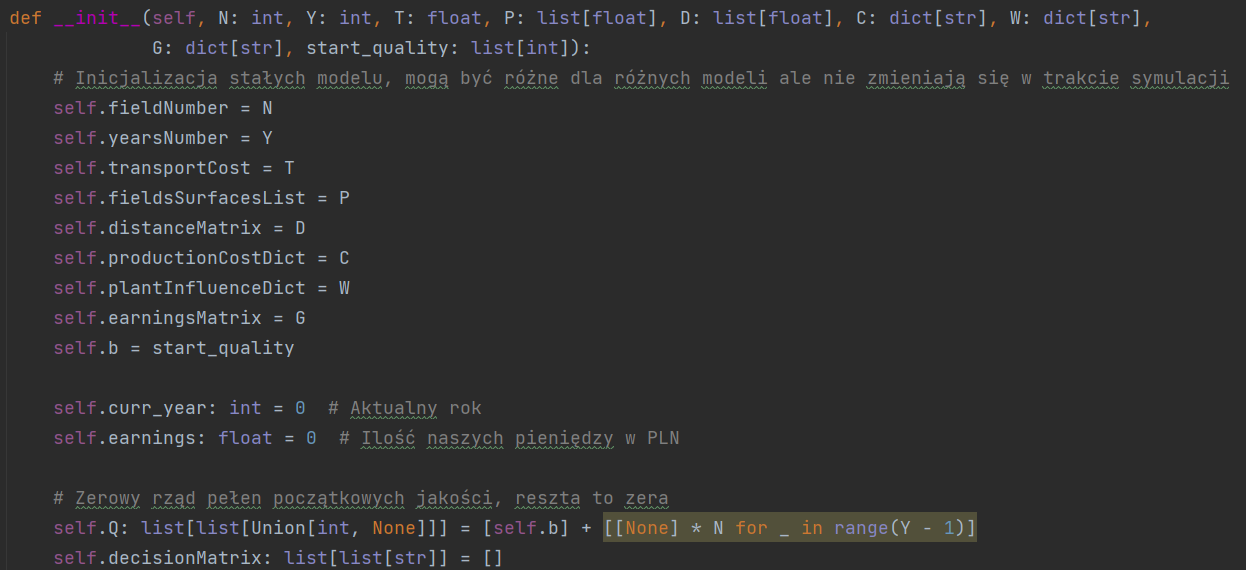
\includegraphics[width=1.1\linewidth]{screens/farm_class.png}
	\caption{init funkcji modelu}
	\label{fig:init}
\end{figure}
\begin{figure}[H]
	\centering
	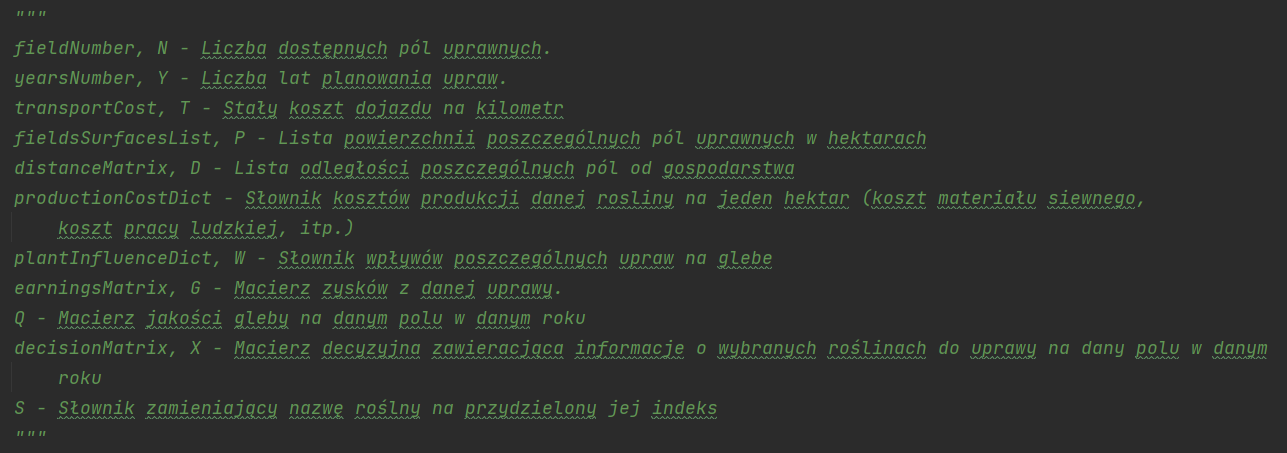
\includegraphics[width=1\linewidth]{screens/oznaczenia}
	\caption{oznaczenia}
	\label{fig:oznaczenia}
\end{figure}



\begin{figure}[H]
	\centering
	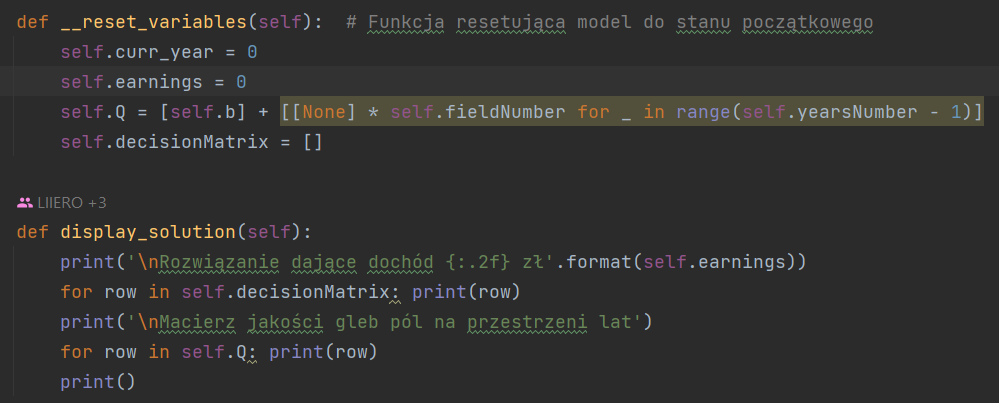
\includegraphics[width=1\linewidth]{screens/funkcje_pom}
	\caption{funkcje pomocnicze}
	\label{fig:funkcjepom}
\end{figure}


\begin{figure}[H]
	\centering
	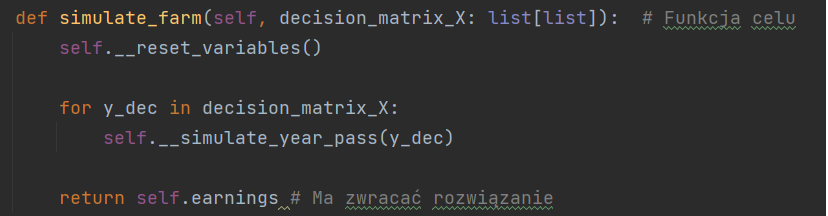
\includegraphics[width=1\linewidth]{screens/stm_farmy}
	\caption{symulacja farmy}
	\label{fig:stmfarmy}
\end{figure}

\begin{figure}[H]
	\centering
	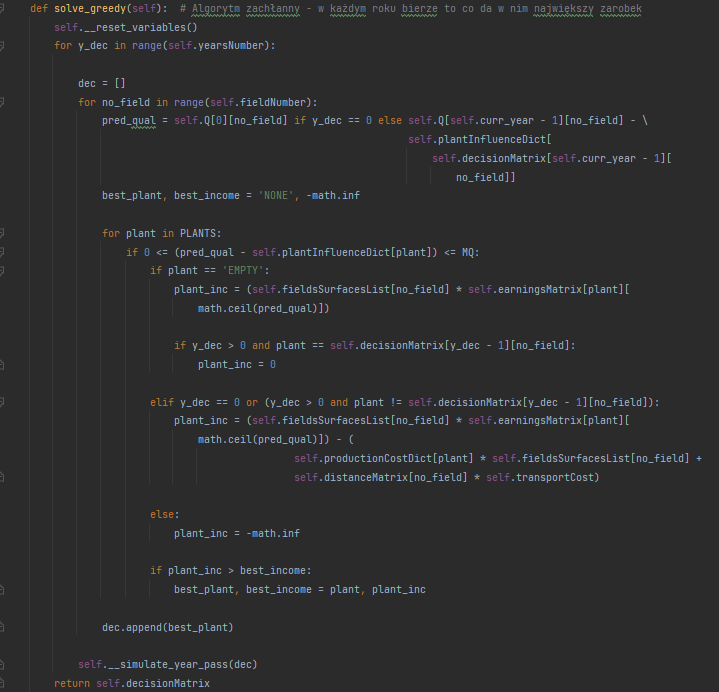
\includegraphics[width=1\linewidth]{screens/greedy}
	\caption{}
	\label{fig:greedy}
\end{figure}


\subsection{symulowane wyżarzanie}
 Nasz problem, na podstawie sugestii pani Profesor postanowiliśmy rozwiązać algorytmem sym. wyżarzania (z ang. simulated anealling). Jest to nasz pierwszy pomysł na rozwiązanie problemu.

\begin{figure}[H]
	\centering
	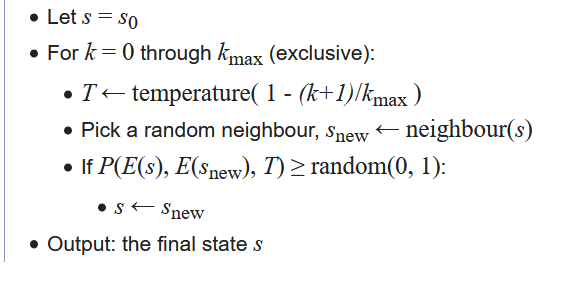
\includegraphics[width=1\linewidth]{screens/pseudocode}
	\caption{}
	\label{fig:pseudocode}
\end{figure}



\begin{figure}[H]
	\centering
	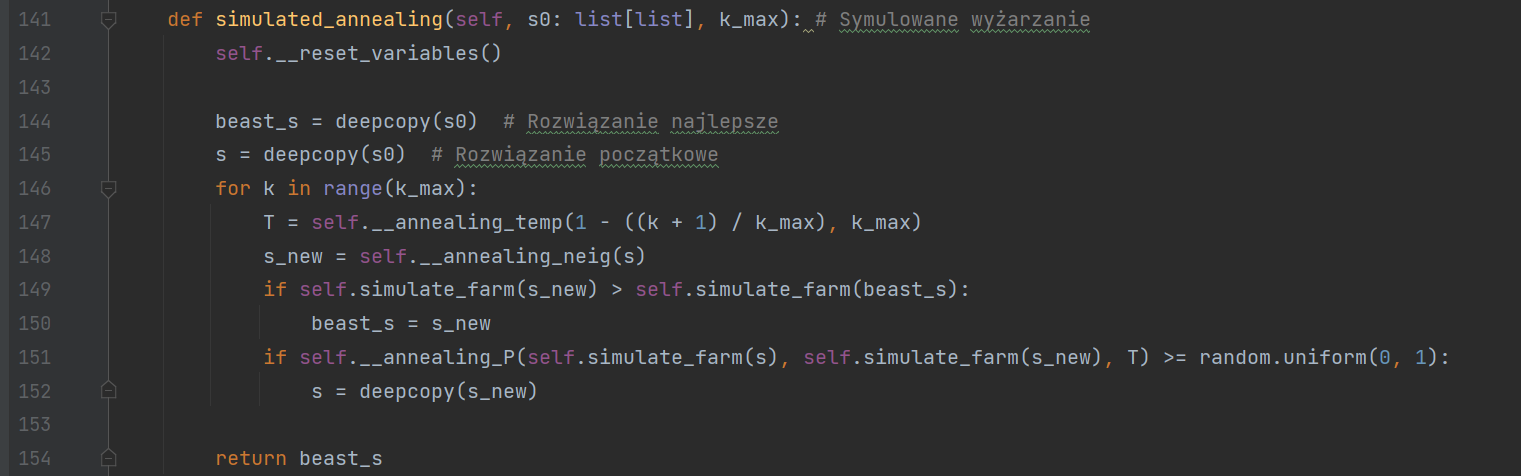
\includegraphics[width=1\linewidth]{screens/anealing_main}
	\caption{główna metoda algorytmu}
	\label{fig:anealingmain}
\end{figure}



\begin{figure}[H]
	\centering
	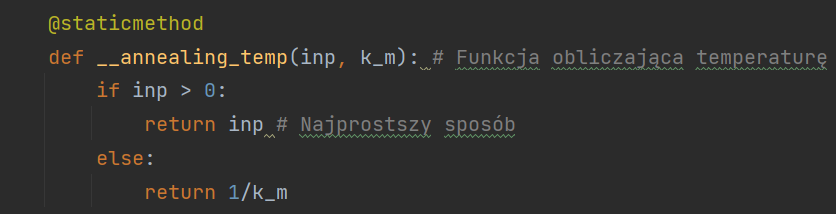
\includegraphics[width=1\linewidth]{screens/anealing_temp}
	\caption{temp}
	\label{fig:anealingtemp}
\end{figure}



\begin{figure}[H]
	\centering
	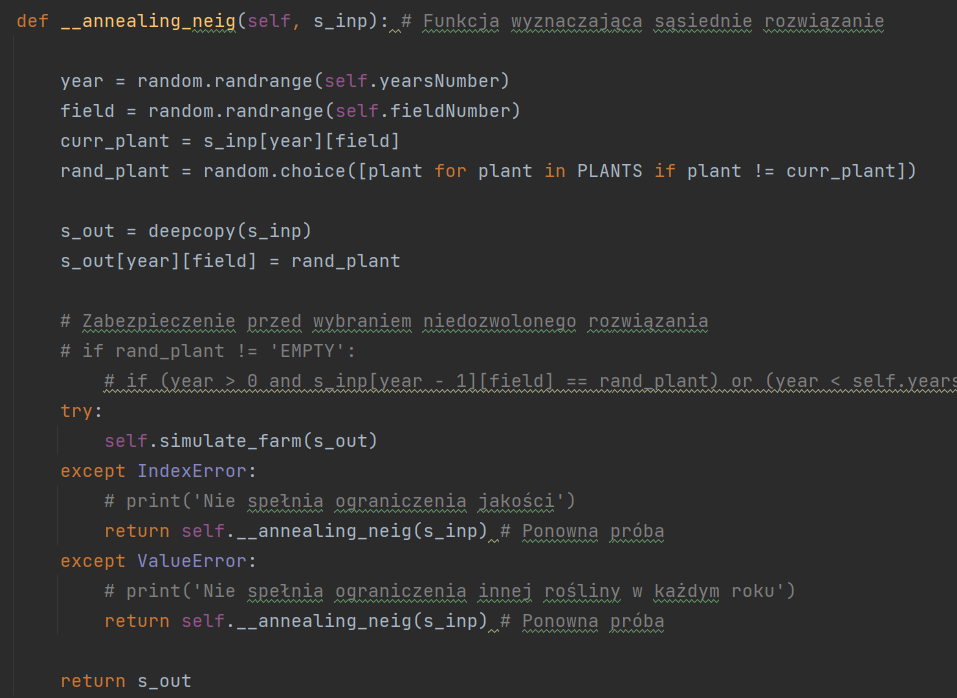
\includegraphics[width=1\linewidth]{screens/anealing_neig}
	\caption{neig}
	\label{fig:anealingneig}
\end{figure}



\begin{figure}[H]
	\centering
	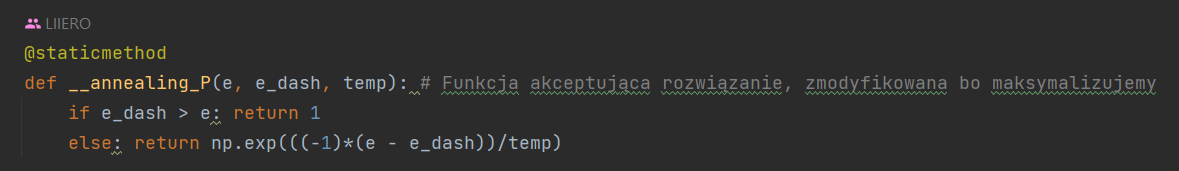
\includegraphics[width=1\linewidth]{screens/anealing_Prob}
	\caption{prob}
	\label{fig:anealingprob}
\end{figure}

\subsubsection{wyniki}

\begin{figure}[H]
	\centering
	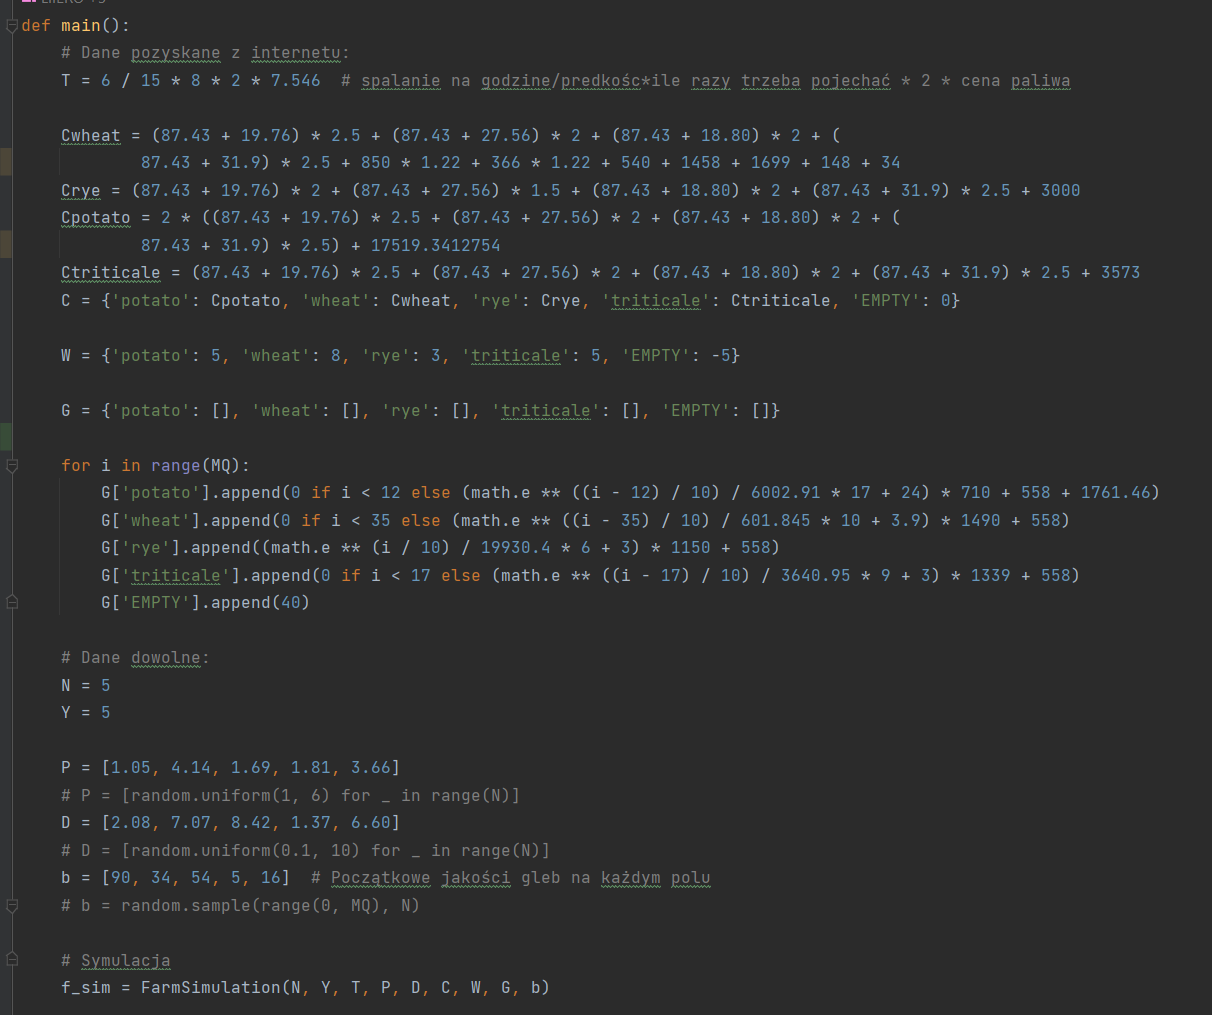
\includegraphics[width=1\linewidth]{screens/main1}
	\caption{Inicjalizacja klasy farm}
	\label{fig:main1}
\end{figure}

\begin{figure}[H]
	\centering
	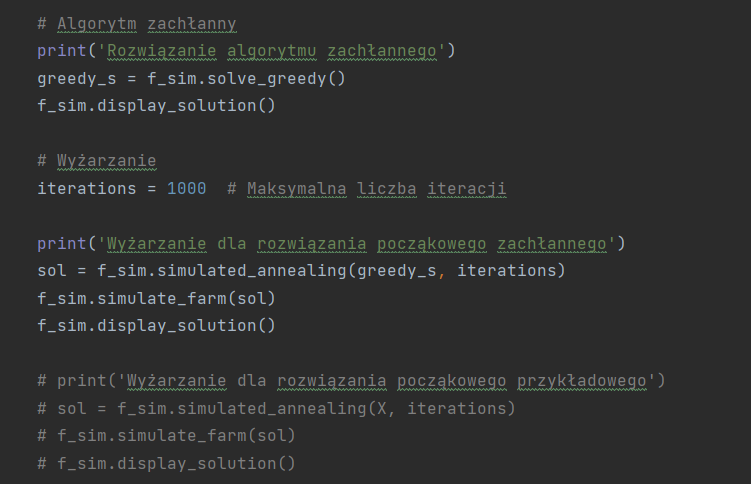
\includegraphics[width=1\linewidth]{screens/main2}
	\caption{}
	\label{fig:main2}
\end{figure}


\begin{figure}[H]
	\centering
	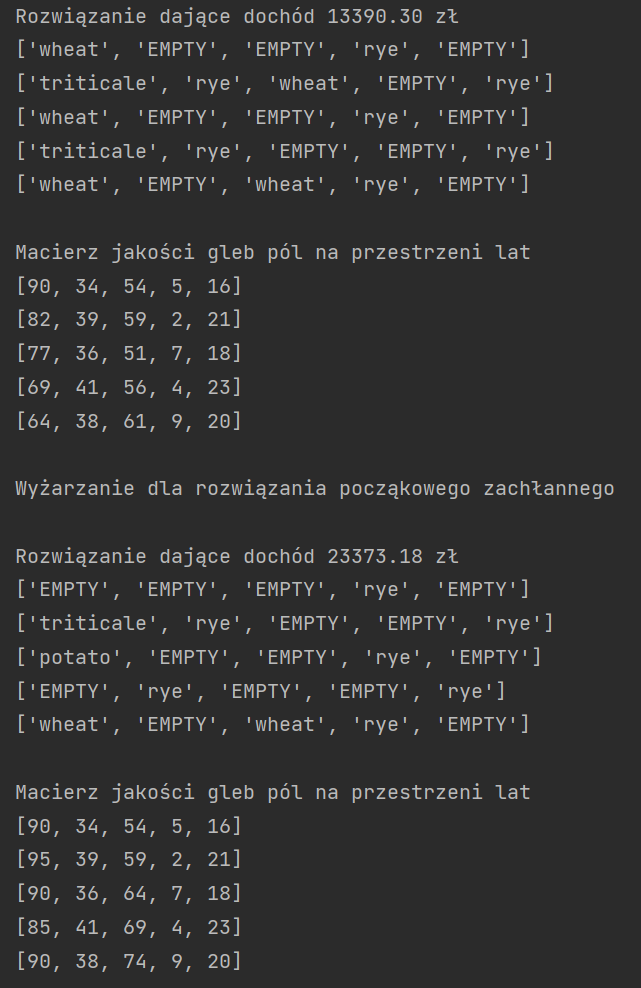
\includegraphics[width=1\linewidth]{screens/przykłądowe_rozw}
	\caption{Rozwiązanie dla przykładowych danych}
	\label{fig:przykadowerozw}
\end{figure}


\section{Inna wersja rozwiązania}

\begin{figure}[H]
	\centering
	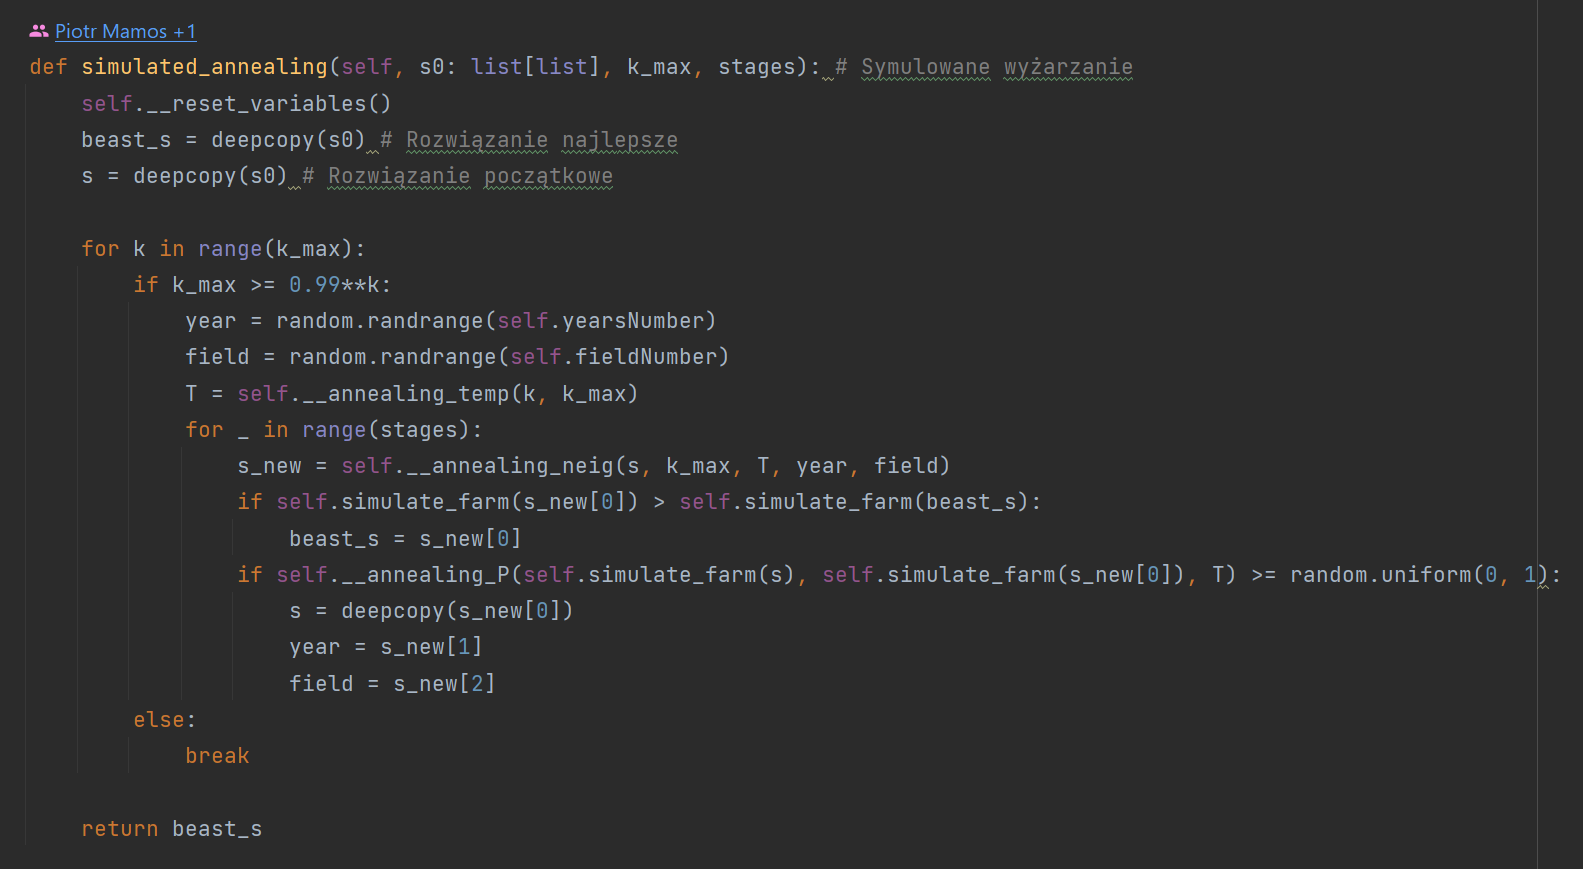
\includegraphics[width=1\linewidth]{screens/mamos_sim_anealing}
	\caption{simulated anealing}
	\label{fig:mamossimanealing}
\end{figure}

\begin{figure}[H]
	\centering
	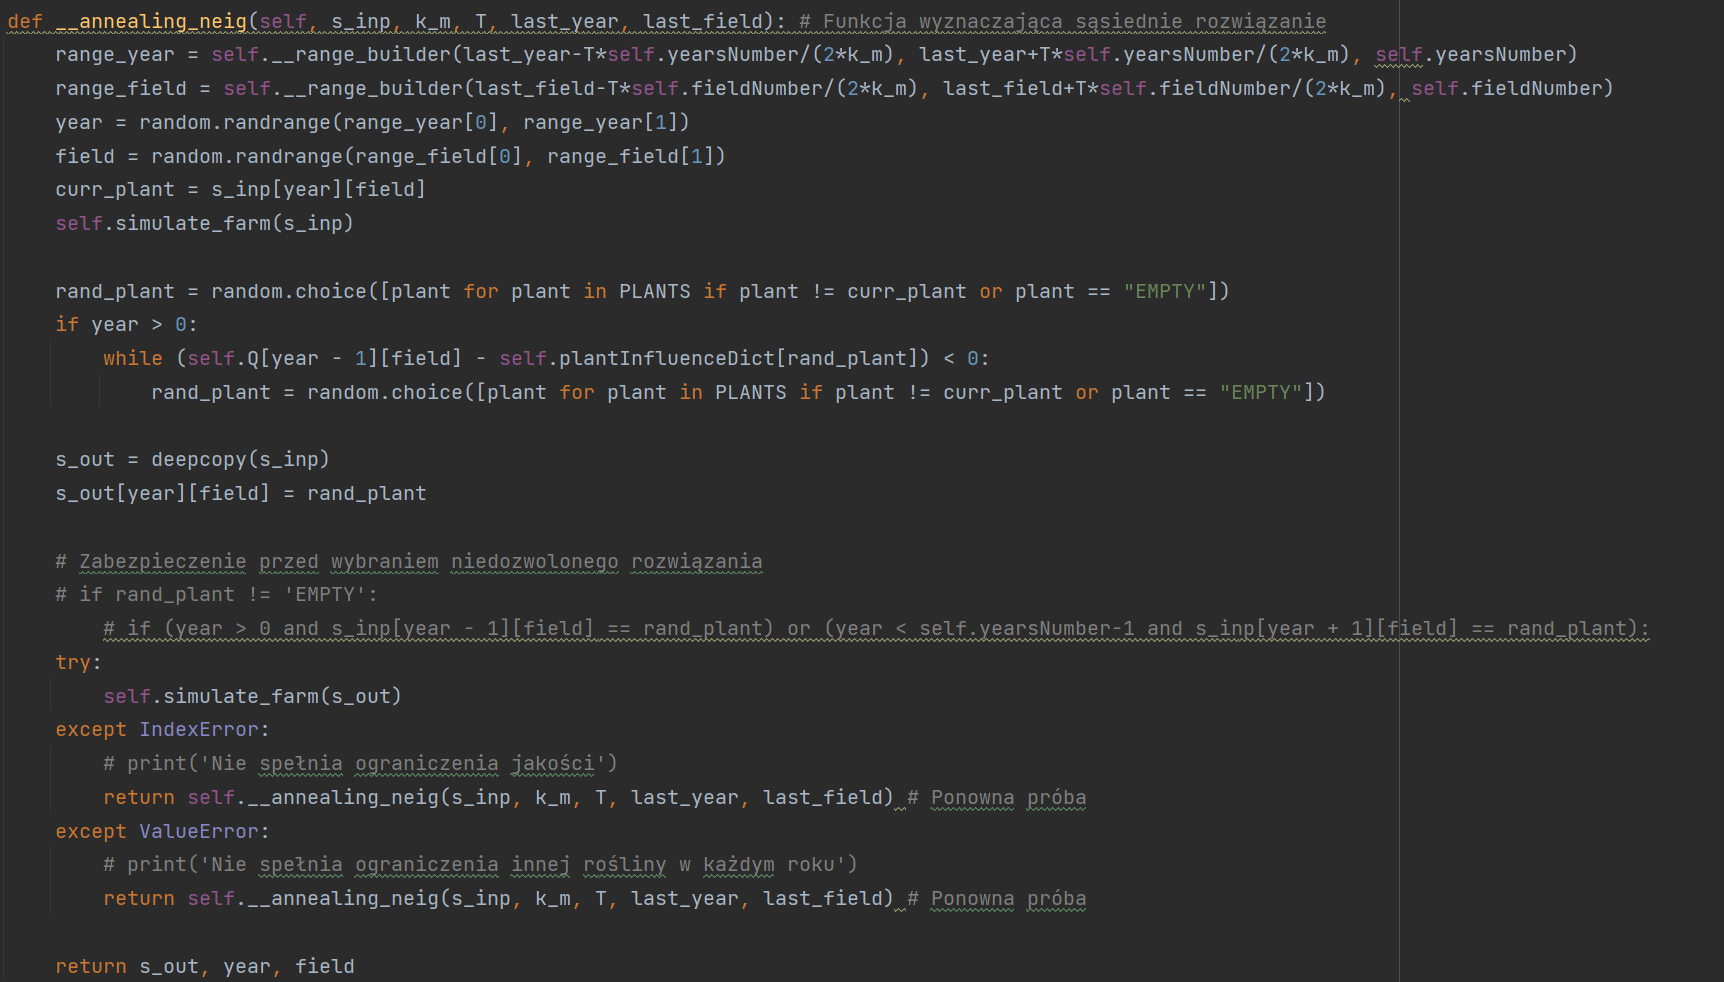
\includegraphics[width=1\linewidth]{screens/mamos_anealing_neig}
	\caption{}
	\label{fig:mamosanealingneig}
\end{figure}

\begin{figure}[H]
	\centering
	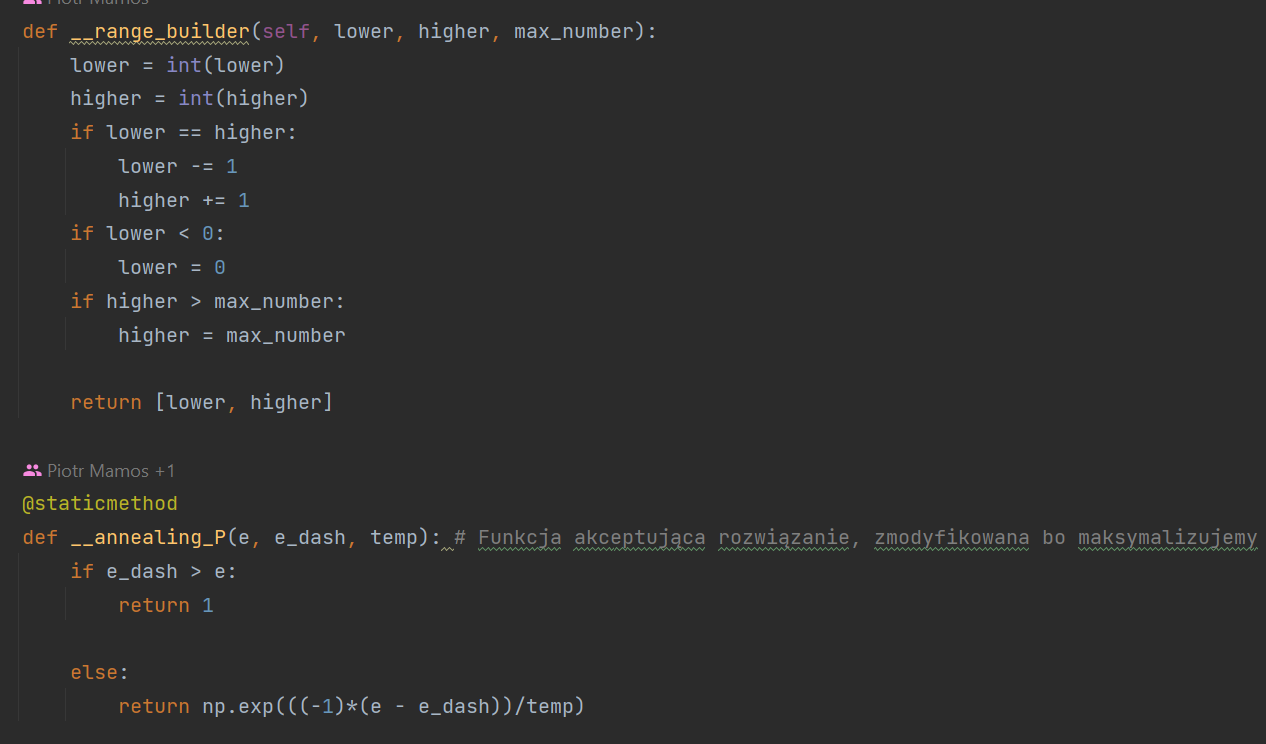
\includegraphics[width=1\linewidth]{screens/mamos_anealing_p_range_builder}
	\caption{}
	\label{fig:mamosanealingprangebuilder}
\end{figure}

\begin{figure}[H]
	\centering
	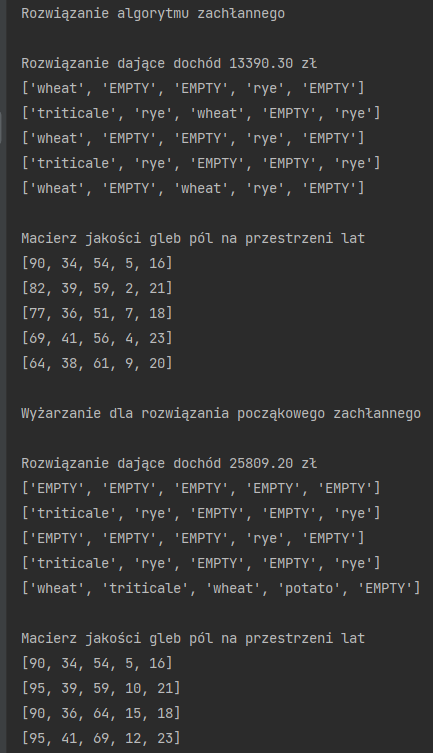
\includegraphics[width=1\linewidth]{screens/mamos_rozw}
	\caption{}
	\label{fig:mamosrozw}
\end{figure}

W porównaniu z naszym pierwszym rozwiązaniem 

\section{Problemy}
	

\end{document}